\documentclass[journal]{IEEEtran}

% *** CITATION PACKAGES ***
\usepackage{cite}

% *** GRAPHICS RELATED PACKAGES ***
%
\ifCLASSINFOpdf
\usepackage[pdftex]{graphicx}
  % declare the path(s) where your graphic files are
  % \graphicspath{{../pdf/}{../jpeg/}}
  % and their extensions so you won't have to specify these with
  % every instance of \includegraphics
  % \DeclareGraphicsExtensions{.pdf,.jpeg,.png}
\else
  % or other class option (dvipsone, dvipdf, if not using dvips). graphicx
  % will default to the driver specified in the system graphics.cfg if no
  % driver is specified.
  % \usepackage[dvips]{graphicx}
  % declare the path(s) where your graphic files are
  % \graphicspath{{../eps/}}
  % and their extensions so you won't have to specify these with
  % every instance of \includegraphics
  % \DeclareGraphicsExtensions{.eps}
\fi
% graphicx was written by David Carlisle and Sebastian Rahtz. It is
% required if you want graphics, photos, etc. graphicx.sty is already
% installed on most LaTeX systems. The latest version and documentation
% can be obtained at: 
% http://www.ctan.org/pkg/graphicx
% Another good source of documentation is "Using Imported Graphics in
% LaTeX2e" by Keith Reckdahl which can be found at:
% http://www.ctan.org/pkg/epslatex
%
% latex, and pdflatex in dvi mode, support graphics in encapsulated
% postscript (.eps) format. pdflatex in pdf mode supports graphics
% in .pdf, .jpeg, .png and .mps (metapost) formats. Users should ensure
% that all non-photo figures use a vector format (.eps, .pdf, .mps) and
% not a bitmapped formats (.jpeg, .png). The IEEE frowns on bitmapped formats
% which can result in "jaggedy"/blurry rendering of lines and letters as
% well as large increases in file sizes.
%
% You can find documentation about the pdfTeX application at:
% http://www.tug.org/applications/pdftex






% *** PDF, URL AND HYPERLINK PACKAGES ***
%
%\usepackage{url}
% url.sty was written by Donald Arseneau. It provides better support for
% handling and breaking URLs. url.sty is already installed on most LaTeX
% systems. The latest version and documentation can be obtained at:
% http://www.ctan.org/pkg/url
% Basically, \url{my_url_here}.


% correct bad hyphenation here
\hyphenation{op-tical net-works semi-conduc-tor}


\begin{document}
%
% paper title
% Titles are generally capitalized except for words such as a, an, and, as,
% at, but, by, for, in, nor, of, on, or, the, to and up, which are usually
% not capitalized unless they are the first or last word of the title.
% Linebreaks \\ can be used within to get better formatting as desired.
% Do not put math or special symbols in the title.
\title{Análisis Acústico de Aullidos y Maullidos}


\author{Álvaro Salgado López}

% note the % following the last \IEEEmembership and also \thanks - 
% these prevent an unwanted space from occurring between the last author name
% and the end of the author line. i.e., if you had this:
% 
% \author{....lastname \thanks{...} \thanks{...} }
%                     ^------------^------------^----Do not want these spaces!
%
% a space would be appended to the last name and could cause every name on that
% line to be shifted left slightly. This is one of those "LaTeX things". For
% instance, "\textbf{A} \textbf{B}" will typeset as "A B" not "AB". To get
% "AB" then you have to do: "\textbf{A}\textbf{B}"
% \thanks is no different in this regard, so shield the last } of each \thanks
% that ends a line with a % and do not let a space in before the next \thanks.
% Spaces after \IEEEmembership other than the last one are OK (and needed) as
% you are supposed to have spaces between the names. For what it is worth,
% this is a minor point as most people would not even notice if the said evil
% space somehow managed to creep in.








% If you want to put a publisher's ID mark on the page you can do it like
% this:
%\IEEEpubid{0000--0000/00\$00.00~\copyright~2015 IEEE}
% Remember, if you use this you must call \IEEEpubidadjcol in the second
% column for its text to clear the IEEEpubid mark.



% use for special paper notices
%\IEEEspecialpapernotice{(Invited Paper)}


\markboth{Procesamiento Y Clasificación de Datos, 13 Marzo 2025}{}

% make the title area
\maketitle



%\IEEEpeerreviewmaketitle



\section{Introducción}
% The very first letter is a 2 line initial drop letter followed
% by the rest of the first word in caps.
% 
% form to use if the first word consists of a single letter:
% \IEEEPARstart{A}{demo} file is ....
% 
% form to use if you need the single drop letter followed by
% normal text (unknown if ever used by the IEEE):
% \IEEEPARstart{A}{}demo file is ....
% 
% Some journals put the first two words in caps:
% \IEEEPARstart{T}{his demo} file is ....
% 
% Here we have the typical use of a "T" for an initial drop letter
% and "HIS" in caps to complete the first word.
\IEEEPARstart
{E}{l} reconocimiento y análisis de sonidos en animales es una herramienta fundamental en bioacústica y en el desarrollo de modelos de clasificación de especies. A lo largo de la historia, los sonidos emitidos por animales han sido objeto de estudio para comprender su comunicación, comportamiento y reacciones ante distintos estímulos. En particular, los perros y los gatos, al ser dos de las especies más comunes en la convivencia humana, han generado un gran interés en la investigación de sus vocalizaciones.

Los aullidos de los perros y los maullidos de los gatos cumplen diferentes funciones comunicativas, desde expresar emociones hasta alertar sobre peligros o buscar atención. Sin embargo, la estructura espectral de estos sonidos puede diferir considerablemente. En este estudio, se comparan los patrones de frecuencia de aullidos de perros y maullidos de gatos utilizando herramientas de procesamiento de señales. El objetivo es identificar las principales diferencias en las frecuencias dominantes de cada sonido y observar posibles coincidencias entre ambas especies. Con este análisis, se busca contribuir al entendimiento de las diferencias y similitudes en la comunicación vocal de estas especies, lo que podría tener aplicaciones en tecnologías de reconocimiento de audio y en estudios sobre el comportamiento animal.
% You must have at least 2 lines in the paragraph with the drop letter
% (should never be an issue)

\section{Metodología}
Para este análisis se utilizaron grabaciones de sonidos de perros y gatos provenientes del conjunto de datos público "Audio Cats and Dogs" disponible en Kaggle. El proceso de análisis se realizó en varias etapas detalladas a continuación:
\begin{itemize}
    \item Carga y lectura de datos: Se seleccionaron archivos de audio representativos de aullidos de perros y maullidos de gatos. Se utilizó la librería librosa en Python para cargar y procesar las señales de audio en formato digital.
    \item Transformada de Fourier (FFT): Se aplicó la Transformada Rápida de Fourier (FFT) a las señales de audio para obtener su representación en el dominio de la frecuencia. Esto permitió analizar la composición espectral de los sonidos y determinar en qué rangos de frecuencia se concentraba la mayor cantidad de energía.
    \item Espectrograma: Se generaron espectrogramas de cada audio para visualizar la evolución de las frecuencias en el tiempo. Esta representación permite identificar patrones característicos en la estructura de los sonidos de cada especie.
    \item Visualización y comparación: Se crearon gráficas que muestran la distribución de frecuencias dominantes en los aullidos de perros y maullidos de gatos. Además, se analizaron las diferencias en la concentración de energía entre ambos sonidos, lo que permitió identificar características específicas de cada vocalización.
\end{itemize}

\section{Resultados}
Los resultados obtenidos muestran diferencias y similitudes entre las señales de audio analizadas:

Forma de onda: Se observó que los maullidos de los gatos tienen una duración mayor en comparación con los aullidos de los perros. Mientras que un maullido suele durar fracciones de segundo con una estructura rápida y definida, los aullidos de los perros tienden a ser mas cortos, con una forma de onda menos extendida. Esta diferencia en la duración podría estar relacionada con la función comunicativa de cada sonido, ya que los aullidos de perros suelen utilizarse en contextos de llamada a distancia o comunicación social prolongada, mientras que los maullidos están más asociados a interacciones rápidas, esto se aprecia en la Fig \ref{fig:forma de onda}
\begin{figure}
    \centering
    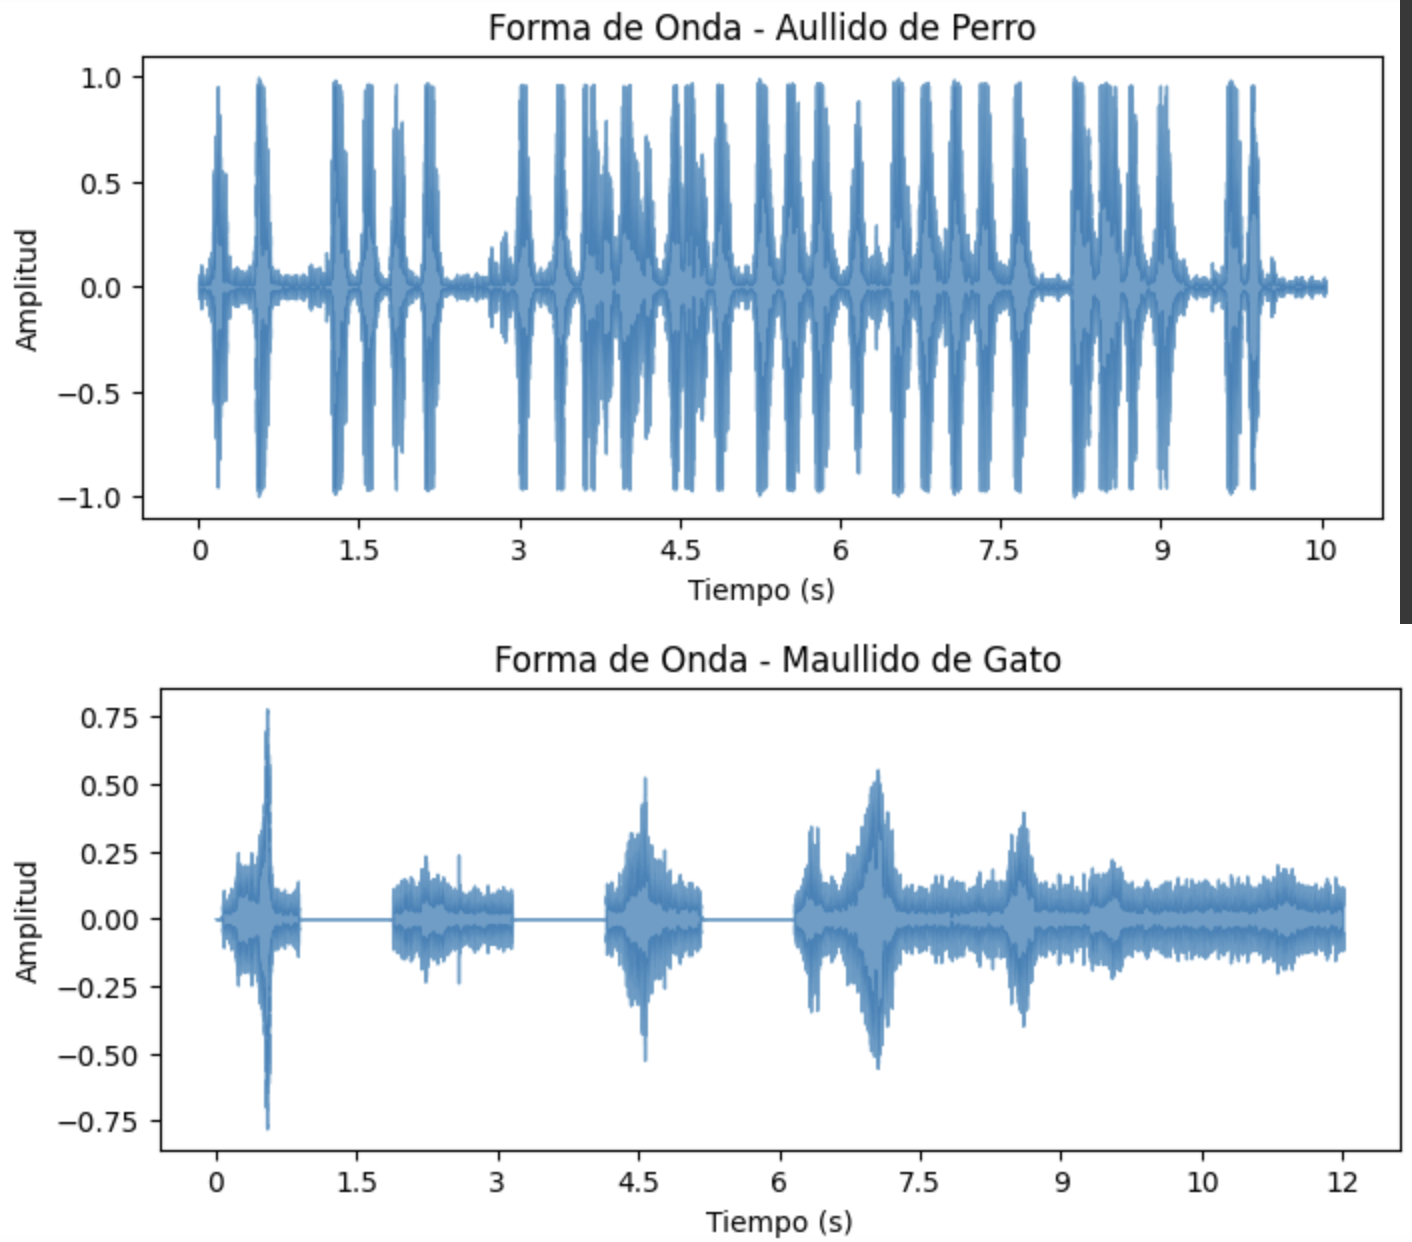
\includegraphics[width=0.5\linewidth]{Figs/Forma de onda.png}
    \caption{Forma de onda}
    \label{fig:forma de onda}
\end{figure}

Espectrograma: El análisis espectral muestra que los aullidos de los perros presentan una mayor cantidad de decibeles (dB) en comparación con los maullidos de los gatos. Esto significa que los aullidos contienen más energía en su emisión y pueden viajar mayores distancias antes de atenuarse. Por otro lado, los maullidos tienden a ser más suaves, con una intensidad menor en comparación. Esto podría estar relacionado con la necesidad de los perros de comunicarse en un rango más amplio, mientras que los gatos utilizan vocalizaciones más enfocadas en interacciones cercanas, esto se observa en la Fig \ref{fig:espectro}

\begin{figure}
    \centering
    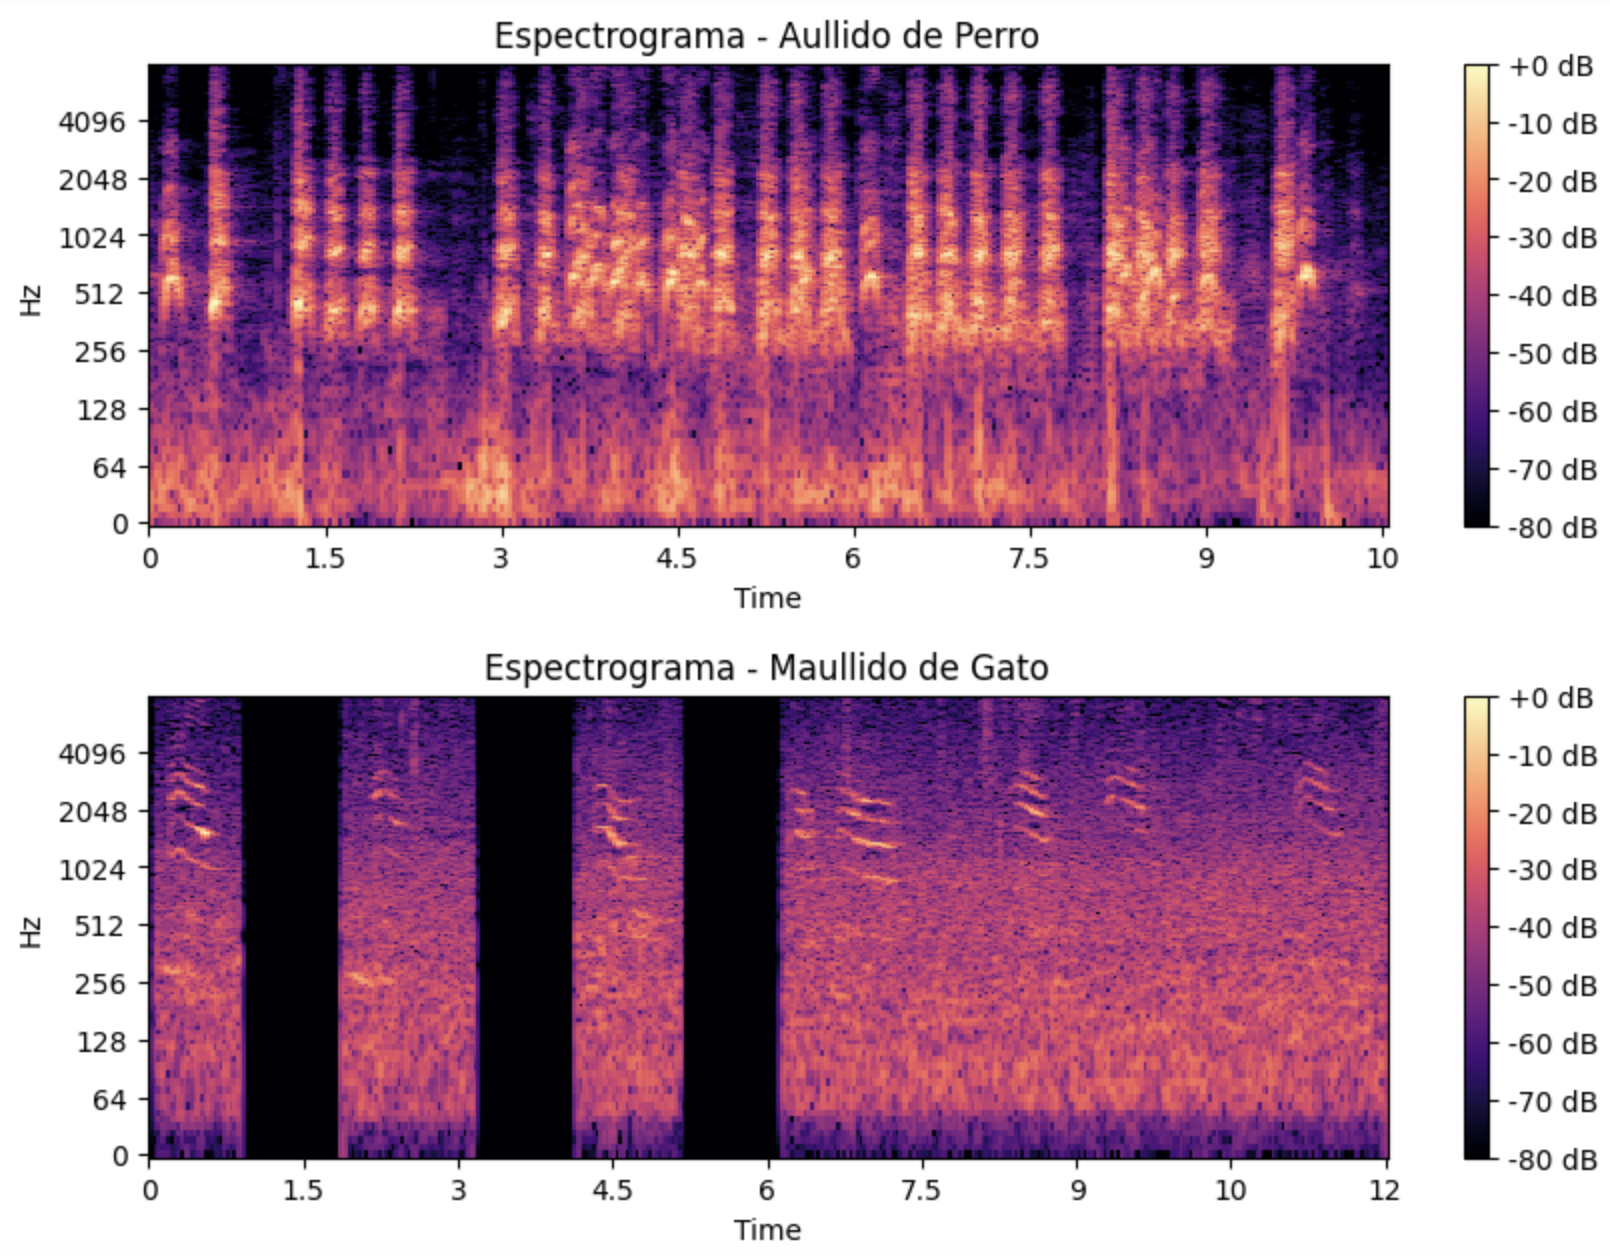
\includegraphics[width=0.5\linewidth]{Figs/Espectro.png}
    \caption{Espectrograma}
    \label{fig:espectro}
\end{figure}

Distribución de frecuencias: En el espectro de frecuencia de los aullidos de los perros, la mayor parte de la energía se concentra en frecuencias entre 200 y 1200 Hz. Este rango se encuentra dentro de los valores característicos de vocalizaciones graves y prolongadas.

En el caso de los maullidos de los gatos, las frecuencias predominantes se encuentran en un rango entre 1000 y 2000 Hz, lo que sugiere una composición más aguda y con una distribución de energía en frecuencias más altas.

Se evidenciaron algunas frecuencias que pueden coincidir entre ambas especies, lo que podría indicar ciertas similitudes en la producción de los sonidos, pero con diferencias marcadas en la intensidad y duración, se aprecia en la Fig \ref{fig:freq}

\begin{figure}
    \centering
    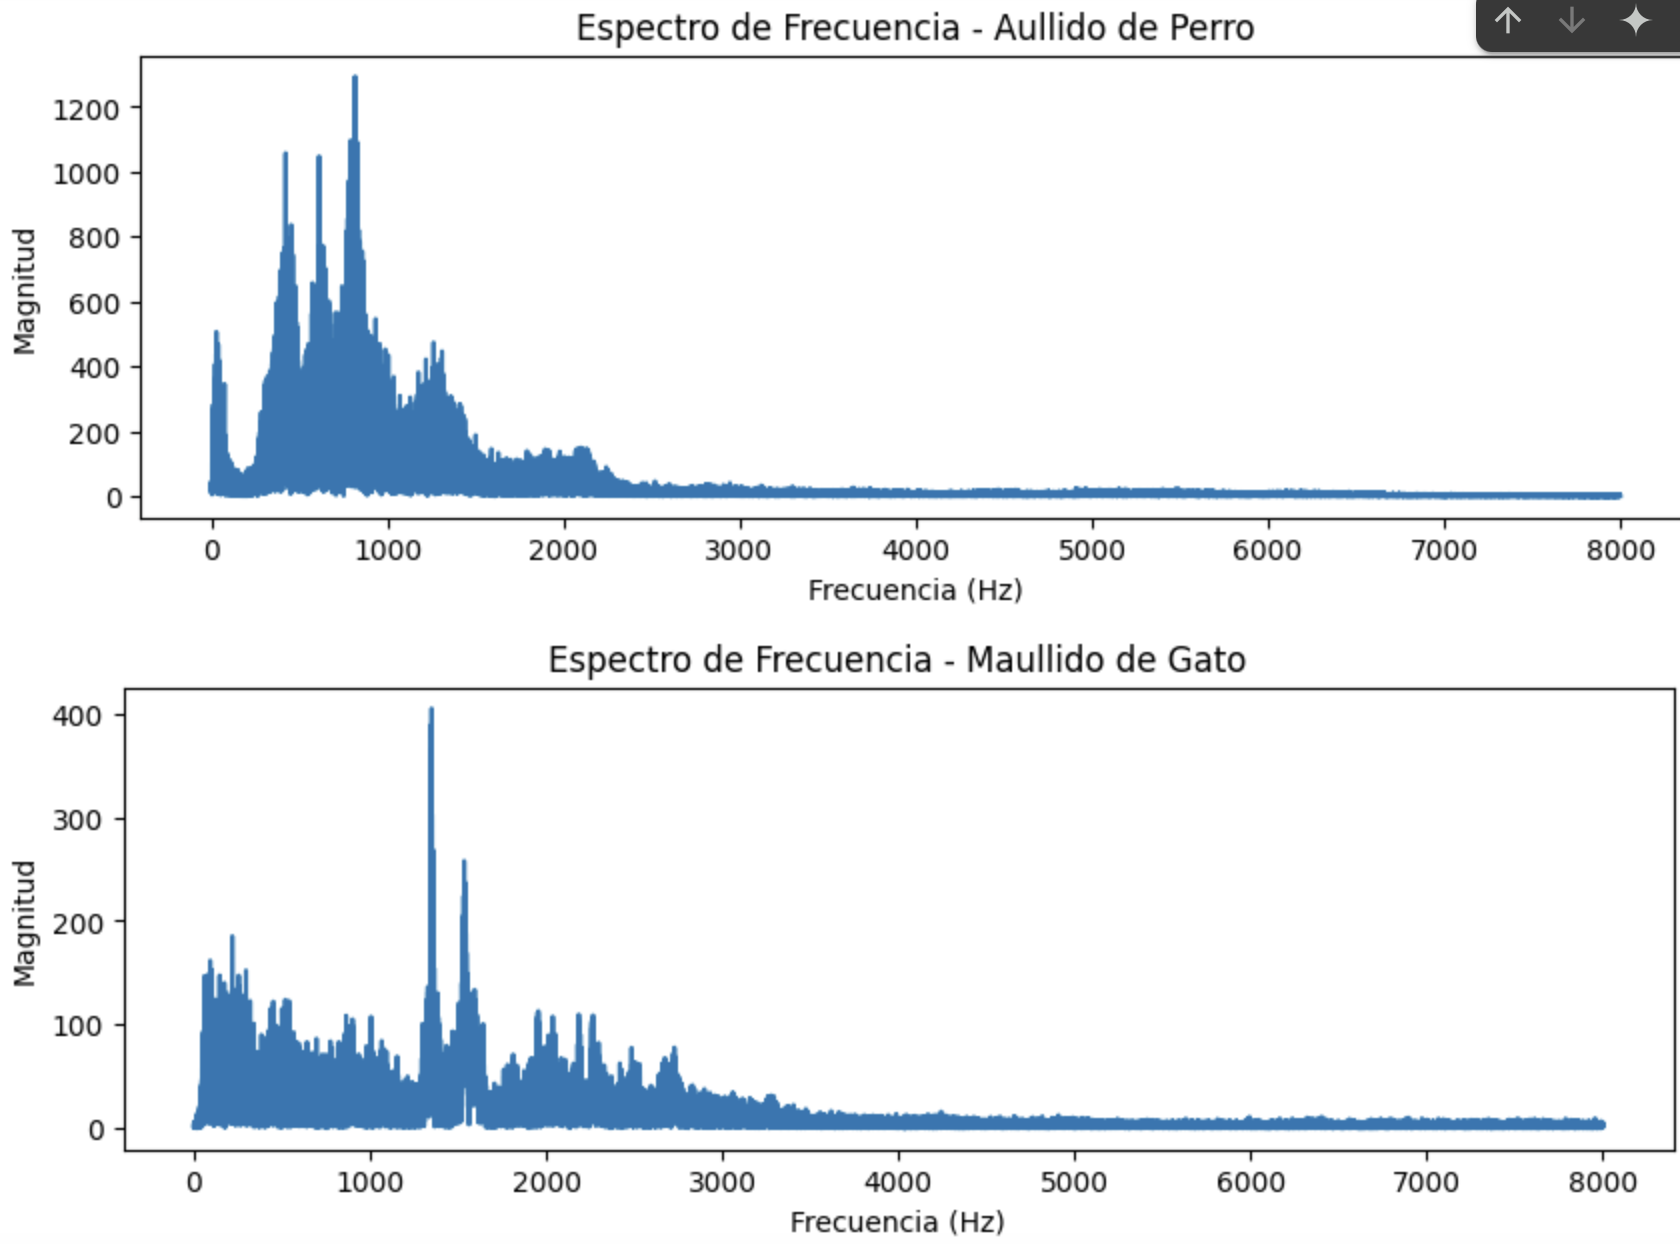
\includegraphics[width=0.5\linewidth]{Figs/freq.png}
    \caption{Espectro de frecuencia}
    \label{fig:freq}
\end{figure}

Estas diferencias observadas pueden tener implicaciones en estudios de clasificación de audio para sistemas de inteligencia artificial, así como en el desarrollo de herramientas para la identificación de especies mediante análisis acústico.

\section{Conclusión}
El análisis espectral de los aullidos de perros y maullidos de gatos demuestra que los perros producen sonidos con frecuencias predominantes en rangos más bajos, mientras que los gatos tienden a emitir sonidos más agudos. Además, los aullidos de perros son de mayor duración e intensidad en comparación con los maullidos de los gatos. Estos hallazgos pueden ser útiles en estudios de clasificación de sonidos, así como en tecnologías de reconocimiento de audio.
% Can use something like this to put references on a page
% by themselves when using endfloat and the captionsoff option.
\ifCLASSOPTIONcaptionsoff
  \newpage
\fi



% trigger a \newpage just before the given reference
% number - used to balance the columns on the last page
% adjust value as needed - may need to be readjusted if
% the document is modified later
%\IEEEtriggeratref{8}
% The "triggered" command can be changed if desired:
%\IEEEtriggercmd{\enlargethispage{-5in}}

% references section

% can use a bibliography generated by BibTeX as a .bbl file
% BibTeX documentation can be easily obtained at:
% http://mirror.ctan.org/biblio/bibtex/contrib/doc/
% The IEEEtran BibTeX style support page is at:
% http://www.michaelshell.org/tex/ieeetran/bibtex/
%\bibliographystyle{IEEEtran}
% argument is your BibTeX string definitions and bibliography database(s)
%\bibliography{IEEEabrv,../bib/paper}
%
% <OR> manually copy in the resultant .bbl file
% set second argument of \begin to the number of references
% (used to reserve space for the reference number labels box)

%\bibliographystyle{IEEEtran} % Estilo de citas de IEEE
%\bibliography{referencias} % Nombre de tu archivo .bib


\end{document}


